\section{Komponenten}
Komponenten, die in vielen anderen Komponenten gebraucht werden, werden bei uns im Ordner
root/components/common gespeichert. Andere Komponenten werden im components-Ordner nach ihrem
zugehörigen Screen getrennt.

\subsection{Snippets}
Um Komponenten schneller erzeugen zu können gibt es in Visual Studio Code Snippets, welche immer den
selben Code generieren.

\begin{figure}[H]
  \begin{center}
    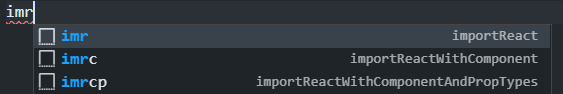
\includegraphics[width=0.5\textwidth]{Mobile/VSSnippets.png}
    \caption{Beispiel für ein Snippet}
  \end{center}
\end{figure}

\begin{figure}[H]
  \begin{center}
    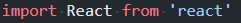
\includegraphics[width=0.5\textwidth]{Mobile/VSSnippetsIMR.png}
    \caption{Vom Snippet erzeugter Code}
  \end{center}
\end{figure}

Da jede Komponente in unserer App ähnlich aufgebaut ist und damit wir nicht jedes mal den gleichen
Code schreiben müssen, habe ich ein eigenes Snippet erstellt. Die Abkürzung rnfec steht für React
Native Functional Component Export Custom und erzeugt folgenden Code:

\begin{code}[htp]
\begin{lstlisting}[firstnumber=1,language=JavaScript, style=JSX]
import React from 'react'
import { View } from 'react-native'
import Text from '@components/common/Text';

const Test = () => {
  return (
    <View>
      <Text></Text>
    </View>
  )
}

export default Test
\end{lstlisting}
\caption{React Component - Snippet rnfec in der Datei Test.js}
\end{code}

Der Name der Komponente wird hierbei vom Dateinamen abgeleitet. Eine Besonderheit, die auffällt, ist
das Import-Statement von Text. Das Verwenden von Alias-Paths wird durch das Babel-Plugin
"module-resolver" möglich gemacht.

\newpage
\subsection{Text}
In React Native gibt es keinen sicheren Weg, um allen Text-Komponenten automatisch eine Font
zuzuweisen, deswegen wird in unserer App immer eine eigene Text-Komponente verwendet. Diese wird
auch beim Erzeugen von neuen Komponenten automatisch eingebunden, damit nicht versehentlich doch die
falsche Komponente verwendet wird.

\begin{code}[htp]
\begin{lstlisting}[firstnumber=1,language=JavaScript, style=JSX]
import colors from '../../styles/Colors';

const CustomText = ({ style, children }) => (
  <Text style={[styles.customFont, style]}>{children}</Text>
);

const styles = StyleSheet.create({
  customFont: {
    fontFamily: 'Poppins-Regular',
    color: colors.text,
  },
});

export default CustomText;
\end{lstlisting}
\caption{React Component - Custom Text Komponente}
\end{code}

Alle Kinder dieser Komponente werden dann direkt in den Text eingebunden und, sollte man noch ein
style-Property an die Komponente übergeben wird der Standard-Style überschrieben.

\newpage
\subsection{Button}
\begin{code}[htp]
\begin{lstlisting}[firstnumber=1,language=JavaScript, style=JSX]
import React from 'react';
import { Pressable } from 'react-native';
import MaterialCommunityIcons from 'react-native-vector-icons/MaterialCommunityIcons';

import Text from './Text';
import styles from '@styles/GlobalStyles';

const Button = ({
  onPress,
  title,
  icon,
  iconType,
  style,
  iconSize = 24,
}) => (
  <Pressable
    onPress={onPress}
    style={[styles.buttonContainer, styles.shadow, style]}
  >
    <Text style={styles.buttonText}>{title}</Text>

    {icon && iconType === 'mci' && (
      <MaterialCommunityIcons
        name={icon}
        size={iconSize}
        color={styles.buttonText.color}
      />
    )}
    ...
  </Pressable>
);

export default Button;

\end{lstlisting}
\caption{React Component - Auch der Button-Component von React Native lässt sich leicht nachbauen.}
\end{code}

Die Funktion, welche beim Drücken aufgerufen werden soll, wird der Komponente als onPress übergeben.
Sollte das Prop icon leer sein, wird kein Icon gerendert, andernfalls wird noch überprüft, welche
Art von Icon verwendet werden soll. Die Icons werden nämlich von mehreren Anbietern bereitgestellt.

\newpage
\subsection{TextInput}
Auch die Komponente TextInput wird von uns überschrieben. Sie besteht zusätzlich immer aus einem
Icon auf der linken Seite. Je nach dem, ob der Input gerade bearbeitet wird, wird die Farbe
verändert. Solle bei der Textüberprüfung ein Fehler auftreten, so wird die Komponente rot gefärbt.

\begin{figure}[H]
  \begin{center}
    
\includegraphics[width=0.5\textwidth]{Mobile/TextInput/unfocused.png}
    \caption{Der TextInput für die Email am Login-Screen}
  \end{center}
\end{figure}

\begin{figure}[H]
  \begin{center}
    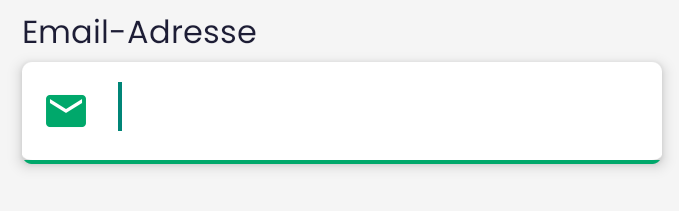
\includegraphics[width=0.5\textwidth]{Mobile/TextInput/focused.png}
    \caption{TextInput ausgewählt}
  \end{center}
\end{figure}

% \begin{figure}[H]
%   \begin{center}
%     
\includegraphics[width=0.5\textwidth]{Mobile/TextInput/error1.png}
%     \caption{Pflichtfeld leer}
%   \end{center}
% \end{figure}

\begin{figure}[H]
  \begin{center}
    
\includegraphics[width=0.5\textwidth]{Mobile/TextInput/error2.png}
    \caption{Fehlerhafte Eingabe}
  \end{center}
\end{figure}

\begin{figure}[H]
  \begin{center}
    
\includegraphics[width=0.5\textwidth]{Mobile/TextInput/valid.png}
    \caption{Korrekte Eingabe}
  \end{center}
\end{figure}